\section{Exercise 3.5 - Master and slave with adapter}

In this exercise we move from the TCL modeling layer to BCAM by implementing a adapter between the master and slave (source and sink) from the previous exercise. The source simply puts data on a FIFO queue, then the adapter is responsible for handling and converting the data to the bus cycle accurate interface on the receiving sink. Figure X exhibits the setup.

\begin{figure}[h]
	\centering
	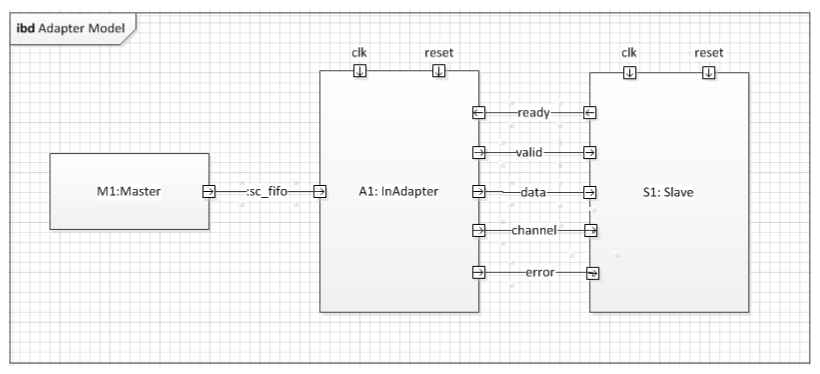
\includegraphics[width=1\linewidth]{MasterSlaveAdapter.png}
	\caption{BCAM model with an adapter in the middle.}
	\label{fig:masterslaveadapter}
\end{figure}

The application file creates instances of the master, slave and the input adapter. We set an appropriate clock, create signals that mimic the ones used in 3.4 and then wire everything together. We introduce a reset and a clock for the adapter to use. It waits for a positive rising edge to sample and write data to the sink. Listing \ref{lst:masterslaveadaptermain} shows the application file.

\begin{lstlisting}[style=customc++, caption=Application file for master/slave with an adapter.,
label={lst:masterslaveadaptermain}]
int sc_main(int argc, char* argv[]) {

	Source Master("Master");
	DataSink Slave("Slave");
	InAdapter<int> inAdapt("instAdapter");
	
	sc_clock clock("clock", sc_time(CLK_PERIODE, SC_NS) ); // 50 MHz
	
	sc_signal<sc_logic> reset;
	sc_signal<sc_logic> ready_channel("C1");
	sc_signal<sc_logic> valid_channel("C2") ;
	
	sc_signal<sc_uint<DATA_BITS> >  data_channel("C3");
	sc_signal<sc_uint<ERROR_BITS> > error_channel("C4");
	sc_signal<sc_uint<CHANNEL_BITS> > channel_channel("C5");
	
	reset = SC_LOGIC_0; // Reset release
	
	Master.out(inAdapt);
	
	inAdapt.valid(valid_channel);
	inAdapt.data(data_channel);
	inAdapt.ready(ready_channel);
	inAdapt.error(error_channel);
	inAdapt.channel(channel_channel);
	inAdapt.clock(clock);
	inAdapt.reset(reset);
	
	
	Slave.valid(valid_channel);
	Slave.data(data_channel);
	Slave.ready(ready_channel);
	Slave.error(error_channel);
	Slave.channel(channel_channel);
	Slave.clk(clock);

	sc_start(2000,SC_NS);
	return 0;
}
\end{lstlisting}

The source has become very simple, as it just pushes arbitrary data onto a FIFO queue in a thread for the adapter to receive. Listing \ref{lst:masterslaveadaptersource} shows the source.

\begin{lstlisting}[style=customc++, caption=Source module that generates data.,
label={lst:masterslaveadaptersource}]
SC_MODULE(Source){

	sc_fifo_out<int> out;
	
	void source_thread(void) {
		while(true){
			out.write(rand() % 65536);
			wait(40,SC_NS);
		}}
	SC_CTOR (Source) {
		SC_THREAD(source_thread)
	}
};
\end{lstlisting}

The adapter is implemented as a template C++ class that inherits the \textit{sc\_fifo\_out\_if} of some type $T$ and \textit{sc\_module} class making it a \textit{SC\_MODULE}. The point of interest is the inherited \textit{write()} method that accepts any type $T$ scalar and convert it to a BCAM model by putting data on specific channels to the sink when it receives the ready signal. Also the reset signal must not have been set. 

\ref{lst:masterslaveadapter}
\begin{lstlisting}[style=customc++, caption=Adapter..,
label={lst:masterslaveadapter}]
	
	template <class T>
	class InAdapter: public sc_fifo_out_if <T>, public sc_module
	{
		public:
		// Clock and reset
		sc_in_clk clock; // Clock
		sc_in<sc_logic> reset; // Reset
	
		// Handshake ports for ST bus
		sc_in<sc_logic> ready; // Ready signal
		sc_out<sc_logic> valid; // Valid signal
	
		// Channel, error and data ports ST bus
		sc_out<sc_uint<CHANNEL_BITS> > channel;
		sc_out<sc_uint<ERROR_BITS> > error;
		sc_out<sc_uint<DATA_BITS> > data;
	
		void write (const T & value)
		{
			if (reset == SC_LOGIC_0)
			{
				// Output sample data on negative edge of clock
				while (ready == SC_LOGIC_0)	{
					wait(clock.posedge_event());
				}
			wait(clock.posedge_event());
			data.write(value);
			channel.write(0); // Channel number
			error.write(0); // Error
			valid.write(SC_LOGIC_1); // Signal valid new data
			wait(clock.posedge_event());
			valid.write(SC_LOGIC_0);
		}
		else wait(clock.posedge_event());
	}
	InAdapter (sc_module_name name_)
	: sc_module (name_)
	{ }
	
	... // Other inherited methods implemented here.
	};
\end{lstlisting}

%TODO: Put in rest of code and results.















s











